\begin{problem}{TST 2026 - Bài 1}{standard input}{standard output}{1 second}{256 megabytes}

Hệ thống đô thị của thành phố XYZ có thể được mô phỏng dưới dạng cây gồm $N$ đỉnh và $N-1$ cạnh. Mỗi đỉnh trên cây tương ứng với một khu dân cư, được đánh số từ $0$ đến $N-1$. Mỗi cạnh trên cây tương ứng với một con đường, được đánh số từ $0$ đến $N-2$. Trong đó, con đường thứ $i$ ($0\le i\le N-2$) nối trực tiếp hai khu dân cư $A_i$ và $B_i$.

Ban quy hoạch đô thị đã chọn ra $K$ tuyến đường để làm các \textbf{tuyến đường trọng điểm}. Các tuyến đường này được đánh số từ $0$ đến $K-1$. Trong đó, tuyến đường trọng điểm thứ $i$ ($0\le i\le K-1$) tương ứng với đường đi ngắn nhất xuất phát từ khu dân cư $U_i$ và kết thúc tại khu dân cư $V_i$.

Trong $Q$ ngày tiếp theo, mỗi ngày ban quy hoạch đô thị sẽ chọn ra một \textbf{tuyến đường tiềm năng}. Trong ngày thứ $i$ ($0\le i\le Q-1$), tuyến đường tiềm năng mà ban quy hoạch chọn sẽ là đường đi ngắn nhất xuất phát từ khu dân cư $X_i$ và kết thúc tại khu dân cư $Y_i$. Tuyến đường này trong ngày thứ $i$ sẽ được coi là \textbf{tuyến đường trọng điểm thứ $K$}. Khi kết thúc ngày, tuyến đường tiềm năng trong ngày đó sẽ không được coi là tuyến đường trọng điểm nữa.

Với mỗi ngày, ban quy hoạch muốn chọn ra một số khu dân cư và đặt trạm tại các khu dân cư đó sao cho:
\begin{itemize}
   \item Với mọi tuyến đường trọng điểm được đánh số từ $0$ đến $K$, luôn có \textbf{ít nhất} một trạm được đặt trên các khu dân cư nằm trên tuyến đường đó.
\end{itemize}

\textbf{Lưu ý:} Ban quy hoạch chỉ muốn mô phỏng phương án đặt trạm. Trên thực tế, ban quy hoạch sẽ không xây dựng bất kỳ trạm nào trong suốt thời gian xét các tuyến đường tiềm năng.

\textbf{Yêu cầu:} Giả sử bạn là một thành viên của ban quy hoạch đô thị, hãy viết một chương trình để giải quyết vấn đề trên.

\InputFile
\textbf{Chi tiết cài đặt}

Thí sinh cần cài đặt hàm sau:

\begin{lstlisting}
vector<int> solve(int N, int K, int Q, const vector<int>& A, const vector<int>& B,
                                       const vector<int>& U, const vector<int>& V,
                                       const vector<int>& X, const vector<int>& Y);
\end{lstlisting}

\begin{itemize}
   \item $N$: Số khu dân cư trên hệ thống đô thị của thành phố XYZ.
   \item $K$: Số tuyến đường trọng điểm được ban quy hoạch đô thị chọn.
   \item $Q$: Số ngày ban quy hoạch đô thị xét tuyến đường tiềm năng.
   \item $A,B$: Hai mảng gồm $N-1$ phần tử, trong đó $A_i$ và $B_i$ ($0\le i\le N-2$) đại diện cho hai khu dân cư có con đường thứ $i$ nối trực tiếp trên hệ thống đô thị.
   \item $U,V$: Hai mảng gồm $K$ phần tử, trong đó $U_i$ và $V_i$ ($0\le i\le K-1$) đại diện cho hai khu dân cư bắt đầu và kết thúc của tuyến đường trọng điểm thứ $i$.
   \item $X,Y$: Hai mảng gồm $Q$ phần tử, trong đó $X_i$ và $Y_i$ ($0\le i\le Q-1$) đại diện cho hai khu dân cư bắt đầu và kết thúc của tuyến đường tiềm năng ban quy hoạch chọn trong ngày thứ $i$.
   \item Hàm này cần trả về một mảng $ans$ bao gồm $Q$ phần tử, trong đó $ans_i$ ($0\le i\le Q-1$) là số trạm tối thiểu cần phải đặt nếu xét ngày thứ $i$.
   \item Hàm này sẽ được gọi $T$ lần, mỗi lần gọi tương ứng với một trường hợp thử nghiệm.
\end{itemize}

\textbf{Lưu ý:}
\begin{itemize}
   \item Chương trình của bạn cần phải khai báo thư viện \texttt{"cstationlib.h"} ở đầu.
   \item Trong chương trình, thí sinh được phép cài đặt các biến, các hàm toàn cục, nhưng không được phép có hàm \texttt{main()}.
   \item Chương trình của bạn không được tương tác trực tiếp với đầu vào chuẩn (stdin) và đầu ra chuẩn (stdout).
\end{itemize}

\textbf{Ràng buộc}

\begin{itemize}
   \item $1\le N,K,Q\le 10^5$
   \item $0\le A_i,B_i\le N-1$ với mọi $i$ từ $0$ đến $N-2$
   \item $0\le U_i,V_i\le N-1$ với mọi $i$ từ $0$ đến $K-1$
   \item $0\le X_i,Y_i\le N-1$ với mọi $i$ từ $0$ đến $Q-1$
   \item $A_i\ne B_i$ với mọi $i$ từ $0$ đến $N-2$
   \item $\sum_N,\sum_K,\sum_Q\le 2\times 10^5$
\end{itemize}

\Scoring
\begin{center}
  \begin{tabular}{|c|c|l|} \hline
    \textbf{Subtask} & \textbf{Điểm} & \textbf{Giới hạn} \\ \hline
    1 & $5$ & $1\le N,K,Q\le 14; T\le 50$ \\ \hline
    2 & $10$ & $\sum_N,\sum_K,\sum_Q\le 500$ \\ \hline
    3 & $10$ & $\sum_N,\sum_K,\sum_Q\le 3000$ \\ \hline
    4 & $20$ & $A_i=i,B_i=i+1$ với mọi $i$ từ $0$ đến $N-2$ \\ \hline
    5 & $55$ & Không có ràng buộc gì thêm \\ \hline
  \end{tabular}
\end{center}


\Note
\textbf{Example}

Xét lần gọi hàm sau:

\begin{lstlisting}
solve(6, 2, 2, {0, 0, 0, 1, 2}, {1, 2, 5, 3, 4}, {3, 4}, {1, 2}, {5, 5}, {0, 1})
\end{lstlisting}

Hệ thống đô thị của thành phố XYZ bao gồm $N=6$ khu dân cư và có thể được mô phỏng theo hình như sau:

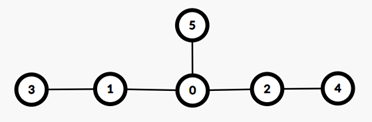
\includegraphics{tst2026-p1-example.png}

Có $K=2$ tuyến đường được ban quy hoạch đô thị chọn làm tuyến đường trọng điểm. Các tuyến đường đó bao gồm:
\begin{itemize}
   \item $3 - 1$
   \item $4 - 2$
\end{itemize}

Ban quy hoạch đô thị sẽ xét tuyến đường tiềm năng trong $Q=2$ ngày tiếp theo:
\begin{itemize}
   \item Trong ngày thứ $0$, tuyến đường tiềm năng là tuyến đường $5 - 0$. Có thể đặt $3$ trạm tại các khu dân cư $3,4,5$ để thỏa mãn yêu cầu đề bài.
   \item Trong ngày thứ $1$, tuyến đường tiềm năng là tuyến đường $5 - 0 - 1$. Có thể đặt $2$ trạm tại các khu dân cư $1,2$ để thỏa mãn yêu cầu đề bài.
   \item Có thể chứng minh không có phương án nào cho ra kết quả tối ưu hơn.
\end{itemize}

Như vậy, hàm trên cần trả về kết quả là $\{3,2\}$.

\end{problem}

